
\chapter{Hodnotenie výslovnosti} \label{cha:mispronunciation-evaluation}

V~rámci tejto kapitoly si priblížime problematiku hodnotenia výslovnosti nenatívnej reči. Na začiatok si obecne popíšeme charakteristiky nenatívnej reči a vymedzíme si dôležité pojmy, ktoré tvoria teoretický základ pre dostatočné pochopenie daných metód. V~ďalšej časti sa zameriame na hodnotenie výslovnosti z~pohľadu výuky cudzích jazykov, čo nám pomôže identifikovať dôležité aspekty, ktoré budú kľúčové pre návrh vlastného systému. Vo zvyšku kapitoly sa potom budeme venovať výlučne automatickému hodnoteniu výslovnosti a popíšeme si jednotlivé prístupy, ktoré sa v~tejto oblasti používajú.

\section{Problematika chybnej výslovnosti}


Chyby vo výslovnosti v~cudzom jazyku (L2) bývajú zapríčinené viacerými faktormi,
avšak najviac ovplyvňuje výslovnosť rečníka jeho materinský jazyk (L1) \cite{Moyer2013}. 
Rozlišujeme dva druhy chýb, segmentálne, označované aj ako fonémické, a prozodické chyby \cite{Witt2012}. % TODO nájsť lepšiu citáciu.
Segmentálne chyby predstavujú substitúcie za iné fonémy, vynechávanie alebo vkladanie foném. Okrem toho môžeme do týchto chýb radiť aj menej závažné chyby, kedy je správna fonéma ako tak vyslovená, avšak je tam stále určitá odlišnosť
od natívnej výslovnosti. Napriek tomu, že sú tieto chyby patrné pre natívneho
rečníka, nemajú vplyv na porozumenie. Vo výuke jazykov preto prevláda názor,
že sú prirodzenou súčasťou prejavu väčšiny rečníkov, a nekladie sa na ne veľký dôraz \cite{Murcia1996}.

Prozodickými chybami rozumieme napr. nesprávny dôraz, rytmus, intonáciu a pod. Dôležitosť prozódie sa líši jazyk od jazyka, zatiaľ čo v~napr. v~slovenčine prozodické chyby nemajú na porozumenie zásadný vplyv, v~tónových jazykoch, ako napr. čínština, môžu viesť až k~zmene významu. 
V~našej práci sa budeme zameriavať výhradne na segmentálne chyby. Pre viac informácii o~prozodických chybách a ich detekcii viď \cite{Witt2012}.

% \begin{note}
%     \begin{itemize}
%        \item Chyby vo výslovnosti v cudzom jazyku bývajú zapríčinené viacerými faktormi, ale najviac ovplyvňuje výslovnosť rečníka jeho materinský jazyk. \cite{TODO}
%        \item Rozlišujeme dva druhy chýb, chyby na úrovni segmentov a prozodické chyby \cite{Moyer2013}.
%        \item Prozodické chyby - dôraz, rytmus a intonácia.
%        \item Chyby na úrovni segmentov predstavujú substitúcie za iné fonémy, vynechávanie alebo vkladanie fonémov. Okrem toho môžeme do týchto chýb radiť aj menej výrazné chyby, kedy je správny foném ako tak vyslovený, avšak je tam stále určitá odlišnosť od natívnej výslovnosti a je teda zrejmé, že daný rečník má akcent. Tieto chyby však nemajú významný vplyv na porozumenie a vo výuke cudzích jazykov nie je na takýto druh braný veľký dôraz. \cite{Murcia1996}.
%        \item V rámci tejto práce sa zameriame na chyby na úrovni segmentov.
%     \end{itemize}
    
% \end{note}

\section{Výuka výslovnosti s~využitím počítača}

Výuka výslovnosti s~využitím počítača (\textit{Computer-assisted Pronunciation Training}, CAPT) môže mať rôzne podoby, od najjednoduchších programov, ktoré užívateľovi ponúkajú audio materiály, cvičenia a pod., až po komplexné systémy, kde používateľ číta zadaný text a systém automaticky ohodnotí jeho výslovnosť. Príklad existujúceho nástroja\footnote{Nástroj SpeechAce dostupný online na adrese ~\url{https://app.speechace.co}.} slúžiaceho na výuku anglickej výslovnosti je možné vidieť na obr. \ref{fig:speechace}.

\noindent Poskytovanie spätnej väzby je pre menej pokročilých študentov veľmi dôležité, nakoľko majú značné problémy s~identifikovaním vlastných chýb \cite{Dlaska2008}.
Neri. a kol. \cite{Neri2006} pozorovali výrazné zlepšenie výslovnosti u~študentov používajúcich nástroj, ktorý vyznačoval zle vyslovené fonémy, v~porovnaní so študentmi, ktorý si mali možnosť iba porovnávať svoju nahrávku s~referenčnou. K~podobným záverom dospeli aj ďalšie práce \cite{Precoda2000, Tanner2009}. Ďalšie zlepšenie výuky by mohlo priniesť diagnostikovanie druhu chyby, napr. že bola vyslovená fonéma /\textturnv/ namiesto fonémy /\ae/. Takáto spätná väzba by však už vyžadovala oboznámenie študentov so základmi fonetiky a fonológie daného jazyka, aby mohli takúto informáciu využiť vo svoj prospech. Preto by bolo asi vhodnejšie túto informáciu štylizovať skôr do podoby nápovedy, napr. požiadať užívateľa, aby pri vyslovení tejto fonémy výraznejšie otvoril ústa.

Nemenej dôležitým aspektom týchto systémov je ich presnosť, nakoľko mylné hodnotenie výslovnosti by mohlo užívateľov miasť a čoskoro ich od používania takýchto nástrojov celkom odradiť \cite{Neri2006}.

% Zároveň je dôležitá aj forma tejto spätnej väzby. Ukázalo sa totiž, že čím
% je detailnejšia, tým má lepší efekt na zlepšenie výslovnosti.

\begin{figure}[h]
    \centering
    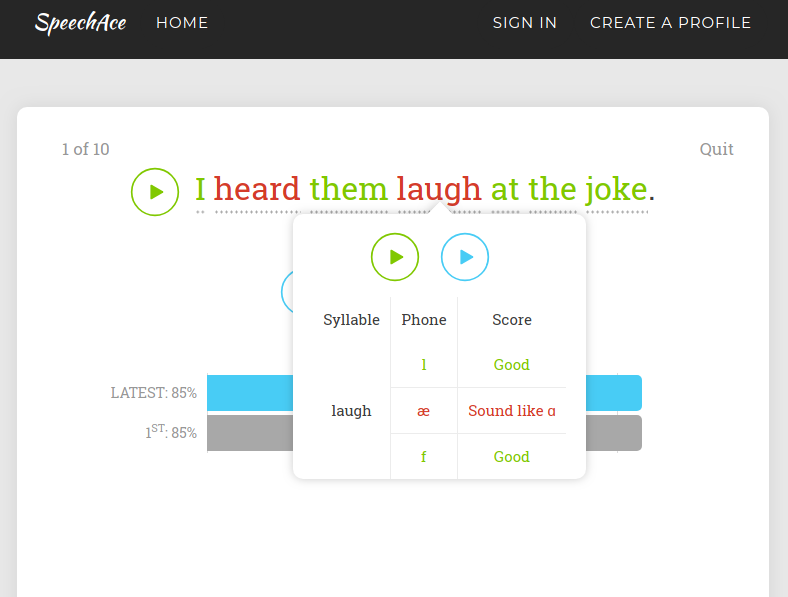
\includegraphics[width=0.9\textwidth]{figures/speechace.jpg}
    \caption{Webové rozhranie nástroja SpeechAce, ktorý slúži na výuku anglickej výslovnosti. Nástroj umožňuje detekciu a diagnostiku segmentálnych chýb. Zle vyslovené fonémy sú označené a je poskytnutá informácia, za aký foném boli substituované. Chýba podpora detekcie chýb založených na vkladaní a vypúšťaní foném.}
    \label{fig:speechace}
\end{figure}

\section{Metódy automatického hodnotenia výslovnosti} \label{sec:confidence-measures}

Pod pojmom automatické hodnotenie výslovnosti rozumieme nejaký algoritmus, ktorý priradí každému segmentu reči číselné skóre, ktoré hovorí, do akej miery je daný segment správne vyslovený. Následne sme aplikovaním určitého prahu 
schopný rozhodnúť, že daný segment je alebo nie je správne vyslovený. K~rozdeleniu nahrávky na segmenty potrebujeme poznať text, ktorý by mal v~danej nahrávke odznieť, pomocou čoho je možné vytvoriť kanonický fonémový prepis, čo je prepis na úrovni foném získaný s~využitím výslovnostného slovníka. Samotné rozdelenie na segmenty je potom realizované núteným zarovnaním voči tomuto prepisu s~využitím ASR systému. Akustický model takéhoto ASR trénujeme s~využitím nahrávok od natívnych resp. nenatívnych rečníkov, v~závislosti na použitej metóde. V~prípade nenatívnych nahrávok je niekedy potrebný aj skutočný prepis, čo je prepis na fonémy, ktoré v~nahrávke rečník vyslovil. Zvyčajne sa na jeho tvorbe podieľajú fonetici, ktorý majú skúsenosť s~daným jazykom.

Ako poznamenali v~\cite{Wei2009}, problém hodnotenia výslovnosti je podobný určovaniu miery dôveryhodnosti rozpoznávania (\textit{Confidence Measures}, CM) u~ASR, kde sa určuje miera istoty, že rozpoznaný výsledok je správny. Analogicky ako v~prípade CM \cite{Jiang2005}, môžeme rozdeliť metódy hodnotenia výslovnosti do troch kategórii:

\begin{enumerate}
    \item metódy založené na teste pomerom vierohodností,
    \item metódy založené na aposteriórnej pravdepodobnosti foném,
    \item metódy založené na priamej klasifikácii výslovnosti.
\end{enumerate}

\noindent V~tejto sekcii si podrobnejšie priblížime jednotlivé metódy.

% Medzi prvé práce, ktoré sa zaoberajú hodnotením výslovnosti na úrovni fonémov
% patrí Kim a kol.\cite{Kim1997}, kde zaviedli a porovnávali niekoľko druhov 
% skóre. Najjednoduchšie z nich spočívalo v normalizácii GMM vierohodností dĺžkou
% segmentu, toto ale neviedlo k dobrým výsledkom. Druhé skóre pracovalo s dĺžkou
% jednotlivých segmentov s ohľadom na rýchlosť reči daného rečníka. Tu už korelácia s ručne anotovanými chybami bola výrazne lepšia, avšak táto metrika našla uplatnenie až pri hodnotení výslovnosti s využitím klasifikácie, viď. 
% \ref{sec:classifier-based-scoring}. Najlepšie výsledky vykazovalo skóre
% založené na aposteriórnej pravdepodobnosti. Nakoľko sa stalo základom pre 
% všetky budúce práce v tejto oblasti, bližšie si ho rozoberieme.

\subsection{Metódy založené na teste pomerom vierohodností} \label{sec:llr-score}

Test pomerom vierohodností (\textit{Likelihood-ratio test}) je v~štatistike využívaný na porovnanie dvoch modelov z~hľadiska toho, ako dobre dané modely vyhovujú pozorovaným dátam. Na detekciu nesprávnej výslovnosti ho prvýkrát použil Franco a kol. \cite{Franco1999} zavedením tzv. \textit{log-likelihood ratio} (LLR) skóre, ktoré je založené na pomere vierohodností od dvoch rôznych GMM-HMM modelov $\lambda_M$ a $\lambda_C$. Obidva modely sú natrénované na foneticky anotovanom datasete nenatívnej reči, avšak pri trénovaní modelu $\lambda_M$ boli použité len nahrávky od rečníkov s~veľmi dobrou výslovnosťou blížiacej sa natívnej úrovni, a model $\lambda_C$ na nahrávkach s~nesprávnou, akcentovanou výslovnosťou. Výpočet pre určitý segment reči, ktorý bol získaný
núteným zarovnaním, je potom nasledovný

\begin{equation} \label{eq:llr-score}
    \text{LLR}(p) = \frac{1}{d} \sum_{t = t_0}^{t_0 + d - 1} \left(\log p(y_t|p, \lambda_M) - \log p(y_t|p, \lambda_C) \right),
\end{equation}

\noindent kde $d$ je počet rámcov v~danom segmente, $t_0$ predstavuje počiatočný index segmentu, $p(y_t|p, \lambda_M)$ je vierohodnosť určená modelom $\lambda_M$, že rámec reči $y_t$ zodpovedá fonéme $p$ a analogicky $p(y_t|p, \lambda_C)$ je vierohodnosť určená modelom $\lambda_C$ pre ten istý rámec $y_t$ a fonému $p$. Normalizácia dĺžkou $d$ zabezpečuje konzistentné skóre nezávislé na dĺžke segmentu. Čím je hodnota tohto skóre vyššia, tým je vyššia pravdepodobnosť, že segment je nesprávne vyslovený. % už si som istý

Franco a kol. vo svojej práci \cite{Franco1999} dosiahli pri použití tohto skóre značné zlepšenie v~porovnaní so skóre založeného na aposteriórnej pravdepodobnosti foném, ktoré je popísané v~nasledujúcej sekcii. Veľkou nevýhodou tejto metódy je potreba nenatívneho datasetu, ktorého obstaranie je značne náročné. 
% TODO zistiť, či musí byť aj anotovaný fonetikmi, alebo stačí kanonická transkripcia

% Veľkou nevýhodou však je L1 jazyková závislosť, čo v kombinácii s náročnosťou zaobstarania nenatívneho datasetu viedlo k snahe o nájdenie lepšej alternatívy. Takéto predpoklady má tendenciu spĺňať tzv. GOP skóre. % TODO prepísať to alebo to hodiť až za to.

\subsection{Metódy založené na aposteriórnej pravdepodobnosti foném} \label{sec:posterior-prob-score}

Spoločným menovateľom metód založených na aposteriórnej pravdepodobnosti foném je snaha o~čo najlepšiu aproximáciu pri výpočte aposteriórnej pravdepodobnosti $P(p|O^{(p)})$, že fonéma $p$ odpovedá segmentu reči $O^{(p)}$. Pre získanie vierohodností potrebných k~výpočtu je použitý akustický model, ktorý
je natrénovaný na natívnom datasete, čo je veľkou výhodou týchto metód. Objavujú sa ale aj práce, v~ktorých sa rozhodli pre použitie nenatívneho datasetu \cite{Arora2017} s~fonetickým prepisom od fonetikov.

Tieto metódy sa zvyknú označovať aj ako \textit{Goodness of pronunciation} (GOP) skóre. Hoci tento názov zodpovedal konkrétnej metóde zavedenej v~práci \cite{Witt2000}, postupnými modifikáciami pôvodného výpočtu sa rozšíril na celú triedu týchto metód.

Na tomto mieste si popíšeme originálne GOP skóre zavedené v~\cite{Witt2000}, ktoré sa dodnes v~určitých podobách stále používa. 
Ako už bolo spomenuté, cieľom GOP je teda určenie normalizovanej aposteriórnej pravdepodobnosti, že foném $p$ odpovedá akustickému segmentu $O^{(p)}$, t.j. 

% \begin{align}
    % \text{GOP}(p) \equiv&  \left| \log P(p | O^{(p)}) \right|  / d \\
                %   =& \left| \log \left( \frac{p(O^{(p)} | p) P(p)}{\sum_{q \in Q} p(O^{(p)} | q) P(q)} \right) \right| \bigg/ d \label{eq:gop1},
% \end{align}

\begin{align}
    \text{GOP}(p) \equiv&  \log P(p | O^{(p)})  / d \\
                  =& \log \left( \frac{p(O^{(p)} | p) P(p)}{\sum_{q \in Q} p(O^{(p)} | q) P(q)} \right) \bigg/ d \label{eq:gop1},
\end{align}

\noindent kde $Q$ je množina všetkých foném a $d$ je počet rámcov
akustického segmentu $O^{(p)}$, $P(p)$, resp. $P(q)$, je apriórna pravdepodobnosť fonémy $p$, resp. $q$, určené jazykovým modelom. Ešte pred tým, než si vysvetlíme význam $p(O^{(p)})$, resp. $p(O^{(q)})$, tak si zavedieme dve zjednodušenia zavedením predpokladov, že všetky fonémy sa vyskytujú s~rovnakou pravdepodobnosťou ($P(p) = P(q)$) a sumu v~menovateli je možné aproximovať maximom. Dostávame teda

% \begin{equation} \label{eq:gop2}
    % \text{GOP}(p) = \left| \log \left( \frac{p(O^{(p)} | p)}{\max_{q \in Q} p(O^{(p)} | q)} \right) \right| \bigg/ d.
% \end{equation}

\begin{equation} \label{eq:gop2}
    \text{GOP}(p) = \log \left( \frac{p(O^{(p)} | p)}{\max_{q \in Q} p(O^{(p)} | q)} \right) \bigg/ d.
\end{equation}

\noindent Určenie vierohodnosti $p(O^{(p)}|p)$ v~čitateli prebieha obvyklým spôsobom, t.j. súčinom vierohodností $p(y_t | p)$ po jednotlivých rámcoch $y_t$ daného segmentu 

\begin{equation}
p(O^{(p)} | p) = \prod_{t=t_0}^{t_0+d-1} p(y_t | p),
\end{equation}

\noindent kde $t_0$ je index prvého rámca segmentu $O^{(p)}$ a $p(y_t | p)$ je  vierohodnosť určená akustickým modelom.

V~prípade menovateľa však postupujeme odlišne. Namiesto výpočtu maxima totiž vykonáme nad danou nahrávkou fonémové rozpoznávanie, čím dostaneme najpravdepodobnejší foném $q$, ktorý zodpovedá segmentu $O^{(p)}$. V~prípade zlej výslovnosti sa však stáva, že zarovnanie získané pri rozpoznávaní sa líši od núteného zarovnania. To má za následok, že segmentu $O^{(p)}$ zodpovedá hneď niekoľko foném $q_1, \dots, q_N$, napr. ako je tomu na obrázku \ref{fig:gop-phone-loop}. Z~toho dôvodu určíme výslednú vierohodnosť $p(O^{(p)} | q)$ ako 

\begin{equation}
p(O^{(p)} | q) = \prod_{i=1}^N p(O^{(p)} | q_i).
\end{equation}

\noindent kde jednotlivé vierohodnosti $p(O^{(p)} | q_i)$ získame analogickým spôsobom ako v~prípade čitateľa, t.j. súčinom po jednotlivých rámcoch, avšak s~ohľadom na hranice dané núteným zarovnaním a rozpoznávaním, viď už spomínaný obrázok \ref{fig:gop-phone-loop}.

\begin{figure} 
    \centering
    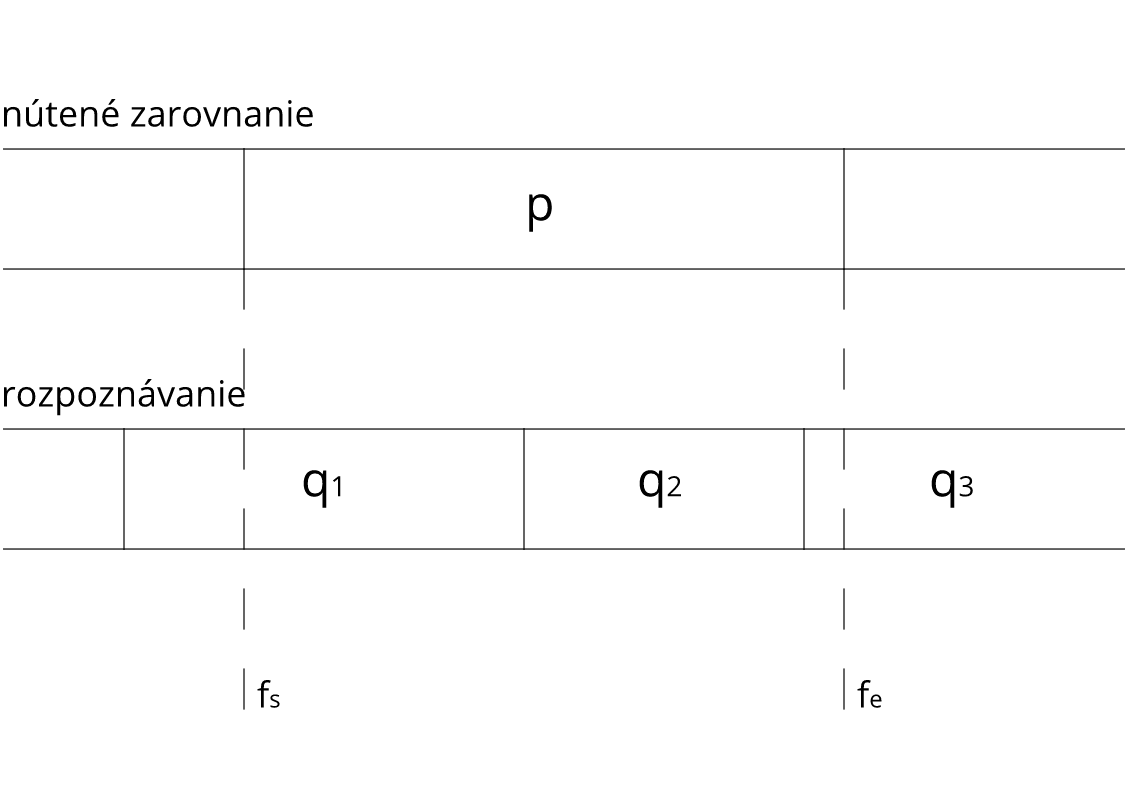
\includegraphics[width=0.6\textwidth]{figures/gop-phone-loop.png}
    \caption{Výsledok zarovnania získaného rozpoznávaním} \label{fig:gop-phone-loop}
\end{figure}

\noindent Tento odlišný výpočet však spôsobí, že skóre môže nadobúdať kladných aj záporných hodnôt, čo by vyžadovalo aj dve prahové hodnoty. Preto vo vzťahu \ref{eq:gop2} aplikujeme na výsledok absolútnu hodnotu, čím dostaneme výsledný vzťah

\begin{equation} \label{eq:gop2}
    \text{GOP}(p) = \left| \log \left( \frac{p(O^{(p)} | p)}{\max_{q \in Q} p(O^{(p)} | q)} \right) \right| \bigg/ d.
\end{equation}

Odteraz nám bude postačovať len jedna hodnota prahu. Narozdiel od predchádzajúceho vzťahu však vyššia hodnota GOP skóre predstavuje horšiu výslovnosť, nie lepšiu.

Toto skóre sa na dlhú dobu stalo de facto štandardom v~hodnotení výslovnosti a v~mnohých prácach sa dodnes používa ako referenčné hodnotenie.
S~rozmachom používania hlbokých neurónových sietí \textit{(DNN -- Deep Neural Network)} bola prirodzene snaha o~ich použitie aj pri výpočte GOP skóre \cite{Hu2013}, čo podľa očakávania viedlo k~obdobnému zlepšeniu ako pri ich použití v~ASR systémoch. 

\subsection{Metódy založené na priamej klasifikácii} \label{sec:classifier-based-scoring}

Veľkou výhodou doposiaľ zmieňovaných metód bola ich jednoduchosť a ľahká realizovateľnosť, nakoľko si vystačili s~existujúcimi časťami bežných ASR systémov. Na druhú stranu však dosahujú pomerne nízku mieru presnosti,
čo môže spôsobovať napr. rovnaký výpočet skóre pre všetky fonémy.
Toto je síce možné čiastočne zlepšiť použitím rôznych prahov pre jednotlivé fonémy \cite{Witt2000}, ale výrazne lepšie dokážu takúto variabilitu pokryť metódy založené na klasifikácii. Tie totiž okrem pravdepodobností z~akustického modelu, ako to bolo u~doterajších metód, využívajú množstvo ďalších príznakov, ako napr. dĺžky segmentov, fonetické vlastnosti a pod. Na základe takýchto informácii sú niektoré klasifikátory potom schopné chyby nielen detekovať, ale aj diagnostikovať, t.j. určiť, o~akú chybu sa jedná. 
% V závislosti na použitých príznakoch sa potom používajú rôzne klasifikátory, napr. LDA, SVM

Prvé použitie klasifikátorov pri hodnotení výslovnosti sa objavilo krátko po zavedení vyššie uvedených metód, kde bola snaha o~ich zlepšenie skombinovaním 
s~ďalšími druhmi metrík, ktoré samostatne nemali veľkú výpovednú hodnotu, ako napr. skóre založené na dĺžke segmentov \cite{Kim1997} a pod. Franco a kol. \cite{Franco2000} porovnávali niekoľko prístupov, ako takúto kombináciu docieliť. Všetky nimi použité klasifikačné metódy dosiahli výrazne lepšie výsledky, ako len pri použití metódy založenej na aposteriornej pravdepodobnosti. K~najlepšej korelácii s~ručne anotovanými hodnoteniami viedlo použitie neurónovej siete alebo rozhodovacieho stromu, kde neurónová sieť dosiahla mierne lepších výsledkov, ale jej trénovanie vyžadovalo ďaleko viac úsilia. 

Širšie využitie však nachádzajú klasifikátory pri úplne odlišnom prístupe, 
kedy sa trénujú nad špecifickými fonémovými pármi, ktoré je v~danom jazyku
potrebné rozlišovať, prípadne stoja za častými chybami vo výslovnosti. 
V~angličtine môže ísť napr. o~dvojicu foném /\textturnv/ a /\ae/. Pre segment obsahujúci jednu z~takýchto foném je klasifikátor schopný určiť, či bola naozaj vyslovená správna fonéma, alebo došlo k~zámene za druhú fonému z~fonémového páru. 
Príkladom takejto práce je napr. \cite{Strik2009}, kde autori trénovali klasifikátory založené na lineárnej diskriminačnej analýze (\textit{Linear Discriminant Analysis}, LDA)
s~využitím niekoľkých akusticko-fonetických vlastností, ktoré boli počítané nad celými segmentmi.
Výsledky, ktoré s~takýmito klasifikátormi dosiahli, výrazne predčili GOP skóre.
K~podobným záverom dospeli aj Doremalen a kol. \cite{Doremalen2009}, ktorý použili SVM klasifikátory pre jednotlivé fonémové páry natrénované nad celou škálou príznakov: logaritmicko-aposteriórne skóre, MFCC príznaky a niekoľko fonetických vlastností.
% Výhodou tohto postupu je možnosť presnejšieho určenia chyby a teda aj možnosť poskytnutia určitej spätnej väzby rečníkovi, ktorá mu môže výrazne napomôcť pri jej odstránení. 
% výrazne prekonať jednoduché metódy založené na aposteriórnej pravdepodobnosti. 



% \begin{note}
%     \begin{itemize}
%         \item Použivajú sa zvyčajne jednoduchšie klasifikačné algoritmy ako LDA alebo SVM, ktoré majú väčšiu tendenciu generalizácie ako napr. neurónové siete.
%     \end{itemize}
% \end{note}

Výskum sa v~posledných rokoch sa začal orientovať na používanie neurónových sietí, či už na samotnú klasifikáciu alebo aj na extrakciu dodatočných príznakov, ako sú napr. fonetické vlastnosti. Pre ilustráciu spomenieme jednu z~týchto prací \cite{Arora2017}, ktorej autori využívajú k~detekcii nesprávnej výslovnosti fonetické vlastnosti, ktorých prítomnosť pre jednotlivé rámce reči určuje hlboká neurónová sieť (\textit{Deep Neural Network}, DNN). Výstupy tejto neurónovej siete vo forme aposteriórnych pravdepodobností sa potom spriemerujú pre celý segment a na základe týchto hodnôt jednouchá neurónová sieť rozhoduje, či je daný segment správne vyslovený. Veľkou výhodou použitia fonetických vlastností je, že v~prípade detekcie nesprávnej výslovnosti máme zároveň detailnú informáciu o~vzniknutej chybe, na základe ktorej je možné rečníka usmerniť, ako danú chybu odstrániť.

% Možným nedostatkom tejto metódy je však spomínané spriemerovanie aposteriórnych pravdepodobností určujúcich fonetické vlastnosti. Po spriemerovaní sa totiž úplne stráca informácia o~zastúpení fonetických vlastností v~čase, čo ale môže byť pri mnohých vlastnostiach kľúčová informácia pre dodatočnú klasifikáciu výslovnosti. Vhodným riešením tohto problému sa javí spôsob popísaný v~práci \cite{Li2017}, ktorá taktiež pojednáva o~detekcii nesprávnej výslovnosti s~využitím fonetických vlastností. Autori namiesto jednoduchého spriemerovania používajú rekurentnú neurónovú sieť, ktorá pre sekvenciu príznakov $x = {x_1, x_2, \dots, x_T}$ predikuje príznakový vektor $y$, ktorý má pre rôzne dĺžky $T$ rovnakú veľkosť. 

% Niektoré chyby však môžu viesť na foném, ktorý sa v danom jazyku vôbec nevyskytuje a preto takto vzniknutý fonémový pár vyžaduje pre trénovanie
% aj nenatívny daset.


% Veľkou výhodou väčšiny systémov založených na výpočte aposteriórnej 
% pravdepodobnosti je ich nezávislosť na natívnom jazyku rečníka. Na druhú stranu takéto Ako sme si však 
% už ukázali v sekcii \ref{sec:llr-score}, zakomponovanie informácie o natívnom
% jazyku rečníka je schopné výrazne zlepšiť schopnosť systému detekovať nesprávnu 
% výslovnosť. 
% Z tohto dôvodu sa ďalší výskum orientoval na prevážne na  
% vývoj metód založených na klasifikácii, ktorá je schopná 

\section{Rozšírené dekódovacie siete}

Rozšírená dekódovacia sieť (\textit{Extended Recognition Network}, ERN) vzniká rozšírením štandardnej dekódovacej siete využívanej v~ASR systémoch o~množinu prechodov zodpovedajúcich chybným výslovnostiam. Takáto sieť môže byť používaná na detekciu nesprávnej výslovnosti bez potreby žiadnej z~uvedených metód v~sekcii \ref{sec:confidence-measures}\cite{Harrison2009, Lo2010}. Zároveň umožňuje okrem detekcie zlej výslovnosti aj jej diagnostiku rozpoznaním chybnej fonémy.  Pri tomto prístupe však nemáme informáciu o~miere istoty, že daný foném je zle vyslovený a nemôžeme tak výslednú chybu nijak ovplyvniť. Najvhodnejšie sa teda ukazuje jej použitie v~kombinácii s~predchádzajúcimi metódami, kedy sa ERN využije len na detekciu chýb spôsobených vložením foném. Na tento typ chýb totiž predchádzajúce metódy nie sú príliš vhodné.

% Vhodnejšie je preto takúto sieť používať pre rozpoznávanie napr. pri výpočte GOP skóre, pretože takéto rozpoznávanie dosahuje výrazne lepšie výsledky ako jednoduchý fonémový rozpoznávač\cite{Harrison2009}. 

K~definovaniu množiny prechodov, o~ktorú sa pôvodná dekódovacia sieť rozšíri, využijeme fonologické pravidlá v~nasledovnom tvare 

\begin{equation}
    \phi \rightarrow \psi / \lambda \_ \, \rho,
\end{equation}

\noindent ktoré hovoria, že fonéma $\phi$ môže byť zamenená za fonému $\psi$ v~prípade, že sa pred ňou nachádza fonéma $\lambda$ a za ňou fonéma $\rho$. Zavedením prázdneho symbolu $\varepsilon$ sme schopní definovať pravidlá chýb spočívajúcich vo vkladaní foném $\varepsilon \rightarrow \psi$ alebo chýb založených na vypúšťaní foném $\phi \rightarrow \varepsilon$. 

Takéto pravidlá je možné pripraviť ručne \cite{Harrison2009} na základe dobrej lingvistickej znalosti oboch jazykov, L1 aj L2. Výsledok takéhoto postupu však bude závislý na autorových znalostiach a bude sa teda výrazne líšiť od autora k~autorovi. Preto vhodnejší spôsob získania týchto pravidiel je pomocou automatického porovnávania prepisov L1 a L2 jazykov \cite{Lo2010}, pričom pre konštrukciu ERN sa použijú  len najčastejšie pravidlá, ktoré pokrývajú určitý počet chýb. Takýto prístup dosahuje výrazne lepšiu úspešnosť pri detekcii zlej výslovnosti, avšak zaobstaranie dostatočne veľkého nenatívneho datasetu je značne náročné.

% \begin{note}
%     \textbf{TODO:}
%     \begin{itemize}
%         \item popísať konštrukciu ERN
%         \item doplniť obrázky s príkladom ERN
%     \end{itemize}
% \end{note}

% Ešte pred tým je však potrebné z WFST reprezentácie siete odstrániť ceny zo všetkých prechodov, t.j. v podstate degradovať túto sieť na FST. 

% \section{Záver}

% V rámci tejto kapitoly sme zhrnuli najdôležitejšie metódy, ktoré .... Obsiahlejší  popis výskumu, ktorý sa odohral v tejto oblasti je možné nájsť v \cite{}
